\documentclass[11pt]{article}

%\usepackage[nosol]{optional}
\usepackage[sol]{optional}

\usepackage {tikz}
    \usetikzlibrary{calc,shapes,arrows,automata,positioning,cd}
    \tikzset{
     dot node/.style={font=\sffamily\small},
      cfgedge/.style   = {black, ->, >=stealth},
      forward/.style = { blue, ->, >=angle 45},
      backward/.style = { red, densely dashed, ->, >=latex' },
      backwardleft/.style = { red, densely dashed, <-, >=latex' },
      position/.style args={#1:#2 from #3}{
        at=(#3.#1), anchor=#1+180, shift=(#1:#2)
    },
    }
    \usepackage{xcolor}

\usepackage{listings, ../listings-rust/listings-rust}
\usepackage{listings}
\usepackage{xcolor}
\definecolor{codegreen}{rgb}{0,0.6,0}
\definecolor{codegray}{rgb}{0.5,0.5,0.5}
\definecolor{codepurple}{rgb}{0.58,0,0.82}
\definecolor{backcolour}{rgb}{0.95,0.95,0.92}
\lstset{
    language=Python,
    keepspaces=true,
    numbers=left,
    backgroundcolor=\color{backcolour},
    commentstyle=\color{codegreen},
    basicstyle=\ttfamily,
    otherkeywords={self,True,False,yield},
    keywordstyle=\ttfamily\color{blue!90!black},
    %basicstyle=\footnotesize,
    keywords=[3]{ttk},
    keywordstyle={[2]\ttfamily\color{orange!80!orange}},
    keywordstyle={[3]\ttfamily\color{red!80!orange}},
    emph={MyClass,__init__},
    emphstyle=\ttfamily\color{red!80!black},
    stringstyle=\color{green!80!black},
    showstringspaces=false
}

\newcommand{\N}{\mathbb{N}}
\newcommand{\Z}{\mathbb{Z}}

% For proof.
\usepackage{amsmath,amsthm,amssymb}

\usepackage{enumerate}
\usepackage{graphicx}
\usepackage{float}
\usepackage{subcaption}
\usepackage{comment}

\renewcommand{\topfraction}{.9}
\renewcommand{\textfraction}{.1}

\usepackage{fullpage,amsmath,amssymb}
\usepackage[colorlinks=true,citecolor=blue,linkcolor=blue]{hyperref} % for href links, and also makes \ref and \eqref clickable in the PDF

% parenthetical comment to state verbally but not write on the board
\newcommand{\com}[1]{\footnote{#1}}

\newcommand{\deltahat}{\widehat{\delta}}

\newcommand{\QuasiP}{\mathsf{QuasiP}}

\newcommand{\TIME}{\mathsf{TIME}}

\usepackage{fancyhdr}
\fancypagestyle{firststyle}
{
    \fancyhf{}
    \fancyhead[C]{Copyright \copyright\ \today, David Doty}
}


\title{Homework 5 \opt{sol}{Solutions} -- ECS 220, Winter 2020}
\date{}
\begin{document}
\maketitle
\thispagestyle{firststyle}
\vspace{-2.0cm}

\section{$2\textsc{Sat}$ is to $\mathsf{NL}$ as $3\textsc{Sat}$ is to $\mathsf{NP}$. (Textbook problem 8.8)}
\begin{quote}
      Show that $2\textsc{Sat}$ is $\mathsf{NL}$-complete.
      {\bf Hint:} first use the discussion in Section 4.2.2 to reduce
      $\textsc{Reachability}$ to the problem $2\textsc{UnSat}$,
      the problem of whether a $2\textsc{Sat}$ formula is unsatisfiable,
      and then use the Immerman-Szelepcs\'{e}nyi Theorem.
      %Can you invent a restricted case of $2\textsc{Sat}$ that is $\mathsf{L}$-complete?
\end{quote}

\section*{Solution}

\subsection*{Reduction}

Given any graph $G = (V, E)$, we want to know if I have a path from  $s \in V$ to $t \in V$.
We are going to convert this problem into $2\textsc{UnSat}$, there is a path iff we can construct a $2\textsc{Sat}$, that cannot be satisfied.

We shall generate a new graph $G'$ that can be converted to a $2\textsc{UnSat}$ clause.

\textbf{The general idea is to consider $s$ adn $t$ as negated values, i.e. $t$ = $-s$, and then mirror the other nodes so it became a symmetric one that can be converted to $2\textsc{UnSat}$.}
Therefore, from now on we may use $-s$ to refer to $t$ and $-t$ to $s$.

\subsubsection*{Convert $G$ to $G'$}

Let's denote $$V = V_{other} \cup \{s, t\}$$.

Then we have: $$V_{other}' = \{-x | x \in V_{other}\}$$

$$V' = V_{other} \cup V_{other}' \cup \{s, t\}$$

Let's denote
$$E_{other} = \{(x, y) | x, y \in V_{other}\}$$
$$E_s = \{(s, x), (y, s) | x, y \in V_{other}, (s, x), (y, s) \in E\}$$
$$E_t = \{(t, x), (y, t) | x, y \in V_{other}, (t, x), (y, t) \in E \}$$

Then we have $$E = E_s \cup E_t \cup E_{other}$$
This way we classified all edges as three types: a) connected(from or to) $s$, b) connetced to $t$, and c) others.

Now let's construct a mirror graph:
$$E_{other}' = \{(-y, -x) | (x, y) \in E_{other}\}$$
$$E_s' = \{(-x, s), (s, -y) | (s, x), (y, s) \in E_s\}$$
$$E_t' = \{(-x, t), (t, -y) | (t, x), (y, t) \in E_t\}$$

$$E' = E_{other} \cup E_{other}' \cup E_s \cup E_s' \cup E_t \cup E_t' $$

This way, we have constructed a new graph $G' = (V', E')$

\subsubsection*{Convert $G'$ to $2\textsc{UnSat}$}

It an be easily seen that if edge $(-x, y)$ exists, $(-y, x)$ must also exist.Therefore we can form a clause $x \vee y$ using the discussion in Section 4.2.2.

Thus we have a full $2\textsc{UnSat}$.

\subsection*{Example}

To give you an example how this reduction works, let's show an example.

\begin{figure}[h]
      \centering
      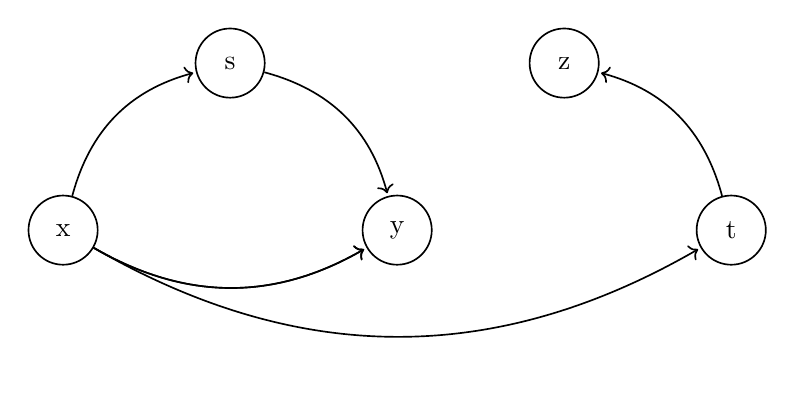
\begin{tikzpicture}[shorten >=1pt,node distance=3cm,on grid,auto, semithick]
            \node [state] (y)                   {y};
            \node [state] (s) [above left of=y]      {s};
            \node [state] (z) [above right of=y]      {z};
            \node [state] (x) [below left of=s]       {x};
            \node [state] (t) [below right of=z]      {t};

            \path[->]
            (x) edge [bend right]   node {} (y)
            (x) edge [bend right]   node {} (t)
            (t) edge [bend right]   node {} (z)
            (s) edge [bend left]   node {} (y)
            (x) edge [bend right]   node {} (y)
            (x) edge [bend left]   node {} (s);
      \end{tikzpicture}
      \caption{An arbitrary graph $G$, clearly there is no path from $s$ to $t$}
\end{figure}

\begin{figure}[h]
      \centering
      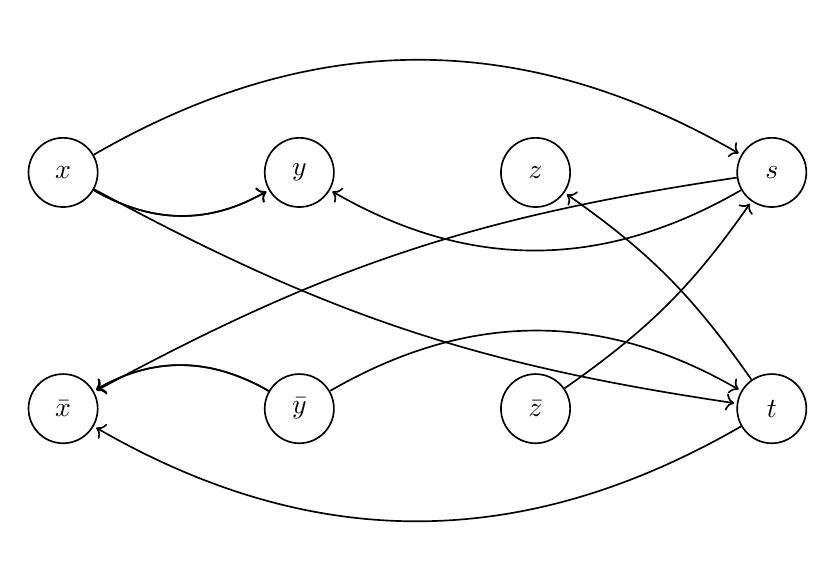
\begin{tikzpicture}[shorten >=1pt,node distance=3cm,on grid,auto, semithick]
            \node [state] (x)                   {$x$};
            \node [state] (y) [right of=x]      {$y$};
            \node [state] (z) [right of=y]      {$z$};
            \node [state] (s) [right of=z]      {$s$};

            \node [state] (nx) [below of=x]      {$\bar{x}$};
            \node [state] (ny) [below of=y]      {$\bar{y}$};
            \node [state] (nz) [below of=z]      {$\bar{z}$};
            \node [state] (t)  [below of=s]      {$t$};

            \path[->]
            (x) edge [bend right]   node {} (y)
            (x) edge [bend right = 10]   node {} (t)
            (t) edge [bend right = 10]   node {} (z)
            (s) edge [bend left]   node {} (y)
            (x) edge [bend right]   node {} (y)
            (x) edge [bend left]   node {} (s)

            (ny) edge [bend right]   node {} (nx)
            (s) edge [bend right = 10]   node {} (nx)
            (nz) edge [bend right = 10]   node {} (s)
            (ny) edge [bend left]   node {} (t)
            (ny) edge [bend right]   node {} (nx)
            (t) edge [bend left]   node {} (nx);
      \end{tikzpicture}
      \caption{The graph $G'$ reduced from $G$}
\end{figure}

Given this graph, the $2\textsc{UnSat}$ generated is:

$$ (-x \vee y) \wedge (-x \vee s) \wedge (-s \vee y) \wedge (-x \vee -s)  $$

\subsection*{Proof of reduction}



\end{document}